\documentclass[tikz,border=5pt, varwidth=false, preview=true]{standalone}
\usepackage{tikz}
\usepackage{enumerate}
\usepackage{enumitem}
\usetikzlibrary{positioning, calc, arrows}
\definecolor{purpleVue}{rgb}{0.6,0.5,0.9}
\usepackage{varwidth}
\begin{document}
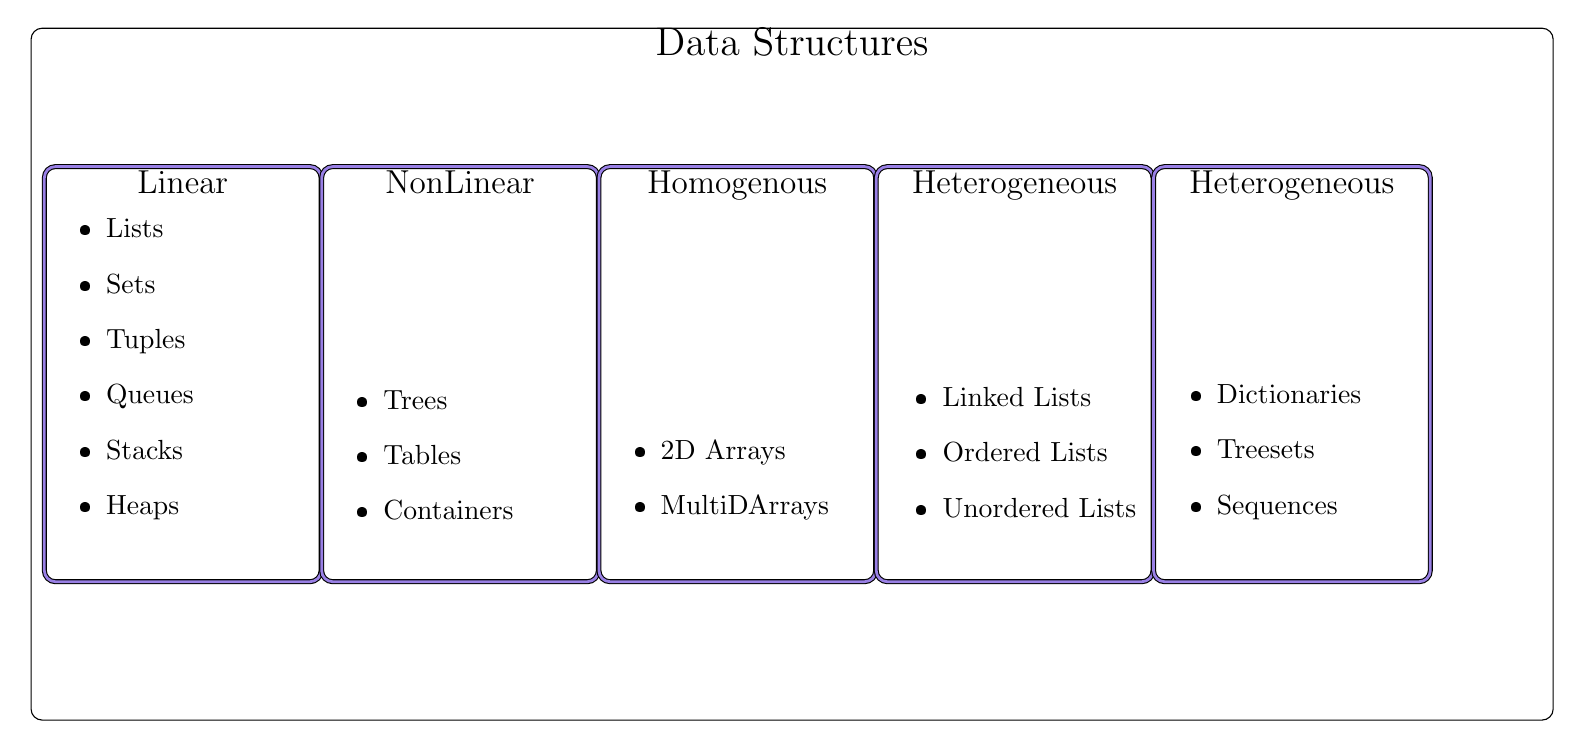
\begin{tikzpicture}[text height=1.5ex,text depth=.25ex]
% Root Node
\node[draw, rounded corners, rectangle, minimum height= 25em, minimum width=55em, label={[anchor=north]north:{\Large Data Structures}}] (DS) {};

% Linear Node
\node[rounded corners, %fill=black,
text depth = 5em, minimum width=10em,
draw,
double=purpleVue, %% here
double distance =1pt,    %% here
%font=\Large, 
minimum height= 15em,
text=purpleVue, label={[anchor=north]north:{\large Linear}}] at ([xshift=5.5em, yshift=0em]
% See https://tex.stackexchange.com/questions/27843/level-of-boldness-changeable
DS.west) (L){};
\node[draw=none] at ([xshift=17em, yshift=-6em] L.west) {{\vbox {
\begin{itemize}
\item Lists
\item Sets
\item Tuples
\item Queues
\item Stacks
\item Heaps
\end{itemize}}
}};

% % Non Linear Node
\node[rounded corners, %fill=black,
text depth = 5em, minimum width=10em,
draw,
double=purpleVue, %% here
double distance =1pt,    %% here
%font=\Large, 
minimum height= 15em,
text=purpleVue, label={[anchor=north]north:{\large NonLinear}}] at ([xshift=5em, yshift=0em]
% See https://tex.stackexchange.com/questions/27843/level-of-boldness-changeable
L.east) (NL){};
\node[draw=none] at ([xshift=17em, yshift=-6em] NL.west) {{\vbox {
\begin{itemize}
\item Trees
\item Tables
\item Containers
\end{itemize}}
}};

% Homogenous Node
\node[rounded corners, %fill=black,
text depth = 5em, minimum width=10em,
draw,
double=purpleVue, %% here
double distance =1pt,    %% here
%font=\Large, 
minimum height= 15em,
text=purpleVue, label={[anchor=north]north:{\large Homogenous}}] at ([xshift=5em, yshift=0em]
% See https://tex.stackexchange.com/questions/27843/level-of-boldness-changeable
NL.east) (Ho){};
\node[draw=none] at ([xshift=17em, yshift=-6em] Ho.west) {{\vbox {
\begin{itemize}
\item 2D Arrays
\item MultiDArrays
\end{itemize}}
}};

% Heterogeneous
\node[rounded corners, %fill=black,
text depth = 5em, minimum width=10em,
draw,
double=purpleVue, %% here
double distance =1pt,    %% here
%font=\Large, 
minimum height= 15em,
text=purpleVue, label={[anchor=north]north:{\large Heterogeneous}}] at ([xshift=5em, yshift=0em]
Ho.east) (He){};
\node[draw=none] at ([xshift=4.5em, yshift=-3em] He.west) {
{
\setlength{\fboxsep}{0pt}%
  \setlength{\fboxrule}{0pt}%
\framebox{\begin{varwidth}{\linewidth}
\begin{itemize}
\item Linked Lists
\item Ordered Lists
\item Unordered Lists
\end{itemize}\end{varwidth}}
}};

% % Heterogeneous
\node[rounded corners, %fill=black,
text depth = 5em, minimum width=10em,
draw,
double=purpleVue, %% here
double distance =1pt,    %% here
%font=\Large, 
minimum height= 15em,
text=purpleVue, label={[anchor=north]north:{\large Heterogeneous}}] at ([xshift=5em, yshift=0em]
He.east) (Dy){};
\node[draw=none] at ([xshift=3.5em, yshift=-3em] Dy.west)  {
{
% This is a better way to set items in a list, such that it doesn't impact the size of the tikzpicture
\setlength{\fboxsep}{0pt}%
  \setlength{\fboxrule}{0pt}%
\framebox{\begin{varwidth}{\linewidth}
\begin{itemize}
\item Dictionaries
\item Treesets
\item Sequences
\end{itemize}\end{varwidth}}
}};
\end{tikzpicture}
\end{document}